\documentclass[compress,11pt,xcolor=svgnames,aspectratio=169]{beamer}
\usetheme{Esiwace}
\usefonttheme[onlysmall]{structurebold}

%\usepackage{caption}
%\captionsetup{labelformat=empty, format=plain, labelsep=none,textfont=footnotesize}

\usepackage[utf8]{inputenc}
\usepackage[english]{babel}
\usepackage[T1]{fontenc}
\usepackage{eurosym}
\usepackage{ulem}
\usepackage{listings}
\usepackage{ragged2e}  %For \justify and \justifying, but it's not working
\usepackage{pgfgantt}
\usepackage{comment}
\usepackage{verbatim}

\tcbuselibrary{raster}
\newcommand{\sectionIntroHidden}{
\begin{frame}{Outline}
  \tableofcontents[currentsection,subsectionstyle=hide/hide/hide]
\end{frame}
}

\DeclareGraphicsExtensions{.pdf,.png,.jpg,}
\graphicspath{{./fig/}}

\title[Summer School -- Input/Output and Middleware -- NetCDF Examples]{Summer School on Effective HPC for Climate and Weather \\[0.5cm] Input/Output and Middleware}
\author[Pedro, Kunkel]{Luciana Pedro, Julian Kunkel
}
\institute[WP4 Team]{Department of Computer Science, University of Reading}
\date{18 June 2020}

\begin{document}

%%%%%%%%%%%%%%%%%%%%%%%%%%%%%%%%%%%%%%%%%%%%%%%%%%%%%%%%%%%%
\begin{frame}[plain]
    \titlepage
\end{frame}

%%%%%%%%%%%%%%%%%%%%%%%%%%%%%%%%%%%%%%%%%%%%%%%%%%%%%%%%%%%%
\begin{withoutheadline}
\begin{frame}{Outline}
    \begin{centering}
    \tableofcontents[hideallsubsections]
    \end{centering}

    \disclaimer
\end{frame}
\end{withoutheadline}

% Input/Output and Middleware
% Climate and weather research is typically data-intensive and applications must utilise input/output efficiently. Often, a user struggles to assess observed performance leading to superflux attempts to tune the application and optimise performance in a wrong layer of the stack. The content of this session is twofold. Firstly, we discuss storage layers focusing on the NetCDF middleware and provide a performance model that aids users to identify inefficient I/O. Secondly, we introduce the NetCDF Climate and Forecast (CF) conventions that are often used as a standard to exchange data.

\begin{frame}[fragile]{Learning Objectives}

\begin{itemize}
  \item Describe the role of middleware and file formats (Section Middleware)
  \item Discuss challenges for data-driven research (Section Data)
  \item Identify typical I/O performance issues and their causes (Section Performance)
  \item Apply performance models to assess and optimize the application I/O performance (Section Model)
  \item Design a data model for NetCDF/CF (Section NetCDF)
  \item Execute programs in C and Python that read and write NetCDF files in a metadata-aware manner (Section Progs)
  \item Analyze, manipulate and visualise NetCDF data (Section NetCDF2)
  \item Implement an application that utilizes parallel I/O to store and analyze data (Section Parallel I/O)
  \item Describe ongoing research activities in high-performance storage (Section Storage)
\end{itemize}

\end{frame}

\section{Building NetCDF}

\begin{frame}[fragile]{Building NetCDF from Scratch}

\begin{itemize}

  \item The usual way of building netCDF requires the HDF5, zlib, and curl libraries.

  \item Files for the libraries can be found in:

\begin{center}
\url{ftp://ftp.unidata.ucar.edu/pub/netcdf/netcdf-4}
\end{center}

\end{itemize}

\end{frame}

\subsection{Installing curl}

\begin{frame}[fragile]{Installing curl}

\begin{itemize}

  \item apt-get install libcurl4-openssl-dev

\end{itemize}

\end{frame}

\subsection{Installing zlib}

\begin{frame}[fragile]{Installing zlib}

\begin{itemize}

  \item wget \url{ftp://ftp.unidata.ucar.edu/pub/netcdf/netcdf-4/zlib-1.2.8.tar.gz}
  \begin{itemize}
    \item Newest version to later use ncview
    \item wget \url{https://sourceforge.net/projects/libpng/files/zlib/1.2.9/zlib-1.2.9.tar.gz}
  \end{itemize}
  \item tar -xvzf zlib-1.2.8.tar.gz
  \item cd zlib-1.2.8
  \item mkdir /home/username/local/
  \item ./configure --prefix=/home/username/local/
  \item make check install

\end{itemize}

\end{frame}

\subsection{Installing HDF5}

\begin{frame}[fragile]{Installing HDF5}

\begin{itemize}

  \item wget \url{ftp://ftp.unidata.ucar.edu/pub/netcdf/netcdf-4/hdf5-1.8.13.tar.gz}
  \item tar -xvzf hdf5-1.8.13.tar.gz
  \item cd hdf5-1.8.13
  \item ./configure --with-zlib=/home/username/local/ --prefix=/home/username/local/
  \item make
  \item make check
  \item make install
  \begin{itemize}
    \item make check install
    \item If not done separately, it might not work!
  \end{itemize}
\end{itemize}

\end{frame}

\subsection{Installing NetCDF}

\begin{frame}[fragile]{Installing NetCDF}

\begin{itemize}

  \item Check the latest version at \url{https://www.unidata.ucar.edu/downloads/netcdf/}
  \item wget \url{ftp://ftp.unidata.ucar.edu/pub/netcdf/netcdf-c-4.7.4.tar.gz}
  \item tar -xvzf netcdf-c-4.7.4.tar.gz
  \item cd netcdf-c-4.7.4
  \item CPPFLAGS=-I/home/username/local/include LDFLAGS=-L/home/username/local/lib ./configure --prefix=/home/username/local
  \item make check install

\end{itemize}

\end{frame}

\begin{frame}[fragile]{Finishing the set up}

\begin{itemize}

  \item Link the NetCDF library\\[0.3cm]
  \begin{itemize}
    \item export \verb|LD_LIBRARY_PATH=/home/username/local/lib/|\\[0.3cm]
    \item \verb|sudo ldconfig|\\[0.4cm]
  \end{itemize}
  \item Create a new directory (for instance, /home/username/example) and create the file from the given source using an editor of your choice.

\end{itemize}

\end{frame}

\section{File \texttt{simple\_xy\_wr.c}}

% Inserting [fragile] to be able to work with \verb

\subsection{Definition}

\begin{frame}[fragile]{File Reference: \texttt{simple\_xy\_wr.c}}

This is an example program demonstrating a simple 2D write. It is intended to illustrate the use of the netCDF C API.\\[0.3cm]

\begin{itemize}
  \item \footnotesize{\url{https://www.unidata.ucar.edu/software/netcdf/docs/simple__xy__wr_8c.html}}\\[0.3cm]
  \item \footnotesize{\url{https://www.unidata.ucar.edu/software/netcdf/docs/simple__xy__wr_8c_source.html}}\\[0.4cm]
\end{itemize}

Dependency graph for \verb|simple_xy_wr|:

\begin{center}
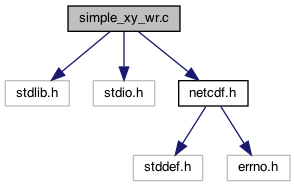
\includegraphics[scale=0.5]{fig/simple__xy__wr_8c__incl}
\end{center}

\end{frame}

\subsection{Code Analysis}

\begin{frame}[fragile]{File \texttt{simple\_xy\_wr.c}: Header and Constants Declaration}

\tiny{

\begin{verbatim}

#include <stdlib.h>
#include <stdio.h>
#include <netcdf.h>

/* This is the name of the data file we will create. */
#define FILE_NAME "simple_xy.nc"

/* We are writing 2D data, a 6 x 12 grid. */
#define NDIMS 2
#define NX 6
#define NY 12

/* Handle errors by printing an error message and exiting with a
* non-zero status. */
#define ERRCODE 2
#define ERR(e) {printf("Error: %s\n", nc_strerror(e)); exit(ERRCODE);}

int
main()
{
  ...
  ...
  ...
}

\end{verbatim}

}

\end{frame}

\begin{frame}[fragile]{File \texttt{simple\_xy\_wr.c}: Variables Declaration}

\tiny{

\begin{verbatim}

...
...
...

int
main()
{
  /* When we create netCDF variables and dimensions, we get back an
   * ID for each one. */
  int ncid, x_dimid, y_dimid, varid;
  int dimids[NDIMS];

  /* This is the data array we will write. It will be filled with a
   * progression of numbers for this example. */
  int data_out[NX][NY];

  /* Loop indexes, and error handling. */
  int x, y, retval;

  ...
  ...
  ...
}

\end{verbatim}

}

\end{frame}

\begin{frame}[fragile]{File \texttt{simple\_xy\_wr.c}: Creating (loading!) data}

\tiny{

\begin{verbatim}

...

int
main()
{
  ...

  /* Create some pretend data. If this wasn't an example program, we
   * would have some real data to write, for example, model
   * output. */
  for (x = 0; x < NX; x++)
     for (y = 0; y < NY; y++)
    data_out[x][y] = x * NY + y;

  ...
}

\end{verbatim}

}

\end{frame}

\begin{frame}[fragile]{File \texttt{simple\_xy\_wr.c}: Creating the NetCDF file}

\tiny{

\begin{verbatim}

...

int
main()
{
  ...

  /* Always check the return code of every netCDF function call. In
   * this example program, any retval which is not equal to NC_NOERR
   * (0) will cause the program to print an error message and exit
   * with a non-zero return code. */

  /* Create the file. The NC_CLOBBER parameter tells netCDF to
   * overwrite this file, if it already exists.*/
  if ((retval = nc_create(FILE_NAME, NC_CLOBBER, &ncid)))
     ERR(retval);

  ...
}

\end{verbatim}

}

\end{frame}

\begin{frame}[fragile]{File \texttt{simple\_xy\_wr.c}: Defining the dimensions}

\tiny{

\begin{verbatim}

...

int
main()
{
  ...

  /* Define the dimensions. NetCDF will hand back an ID for each. */
  if ((retval = nc_def_dim(ncid, "x", NX, &x_dimid)))
     ERR(retval);
  if ((retval = nc_def_dim(ncid, "y", NY, &y_dimid)))
     ERR(retval);

  /* The dimids array is used to pass the IDs of the dimensions of
   * the variable. */
  dimids[0] = x_dimid;
  dimids[1] = y_dimid;

  ...
}

\end{verbatim}

}

\end{frame}

\begin{frame}[fragile]{File \texttt{simple\_xy\_wr.c}: Defining the variable}

\tiny{

\begin{verbatim}

...

int
main()
{
  ...

  /* Define the variable. The type of the variable in this case is
   * NC_INT (4-byte integer). */
  if ((retval = nc_def_var(ncid, "data", NC_INT, NDIMS,
               dimids, &varid)))
     ERR(retval);

  /* End define mode. This tells netCDF we are done defining
   * metadata. */
  if ((retval = nc_enddef(ncid)))
     ERR(retval);

  ...
}

\end{verbatim}

}

\end{frame}

\begin{frame}[fragile]{File \texttt{simple\_xy\_wr.c}: Writing data to the file}

\tiny{

\begin{verbatim}

...

int
main()
{
  ...

  /* Write the pretend data to the file. Although netCDF supports
   * reading and writing subsets of data, in this case we write all
   * the data in one operation. */
  if ((retval = nc_put_var_int(ncid, varid, &data_out[0][0])))
     ERR(retval);

  /* Close the file. This frees up any internal netCDF resources
   * associated with the file, and flushes any buffers. */
  if ((retval = nc_close(ncid)))
     ERR(retval);

  ...
}

\end{verbatim}

}

\end{frame}

\begin{frame}[fragile]{File \texttt{simple\_xy\_wr.c}: Getting SUCCESS!}

\tiny{

\begin{verbatim}

...

int
main()
{
  ...

  printf("*** SUCCESS writing example file simple_xy.nc!\n");
  return 0;
}

\end{verbatim}

}

\subsection{Working and analysing the NetCDF File}

\end{frame}

\begin{frame}[fragile]{Compiling and running the file \texttt{simple\_xy\_wr.c}}

Create (copy!) and compile the file \verb|simple_xy_wr.c|

\begin{itemize}

  \item \tiny{\verb|gcc -I/home/username/local/include simple_xy_wr.c -o simple_xy_wr -L/home/username/local/lib -lnetcdf|}

  \begin{itemize}

    \item What does that mean?!

  \end{itemize}

\end{itemize}

\begin{itemize}

  \item Run the file \verb|simple_xy_wr|

  \begin{itemize}

    \item \verb|./simple_xy_wr|
    \item \verb|*** SUCCESS writing example file simple_xy.nc!|\\[0.5cm]

  \end{itemize}

  \item Check that the file \verb|cmp test.nc simple_xy.nc| is in your directory

    \begin{itemize}

      \item \verb|ls|

    \end{itemize}

\end{itemize}

\end{frame}

\begin{frame}[fragile]{Using \texttt{ncdump}}

Inspect the output file \verb|simple_xy.nc| using \verb|ncdump|

\begin{itemize}

  \item \verb|ncdump simple_xy.nc|

  \item Only works like that in my laptop:

  \item \verb|/home/lucy/netcdf/netcdf-c-4.7.4/ncdump/ncdump simple_xy.nc|

  \item (It should be just ncdump file, but esdm is on my way and I don’t know how to make another link)

\end{itemize}

\end{frame}

\begin{frame}[fragile]{NetCDF CDL Format}

\footnotesize{

\begin{verbatim}

netcdf simple_xy {
dimensions:
	x = 6 ;
	y = 12 ;
variables:
	int data(x, y) ;
data:

 data =
  0, 1, 2, 3, 4, 5, 6, 7, 8, 9, 10, 11,
  12, 13, 14, 15, 16, 17, 18, 19, 20, 21, 22, 23,
  24, 25, 26, 27, 28, 29, 30, 31, 32, 33, 34, 35,
  36, 37, 38, 39, 40, 41, 42, 43, 44, 45, 46, 47,
  48, 49, 50, 51, 52, 53, 54, 55, 56, 57, 58, 59,
  60, 61, 62, 63, 64, 65, 66, 67, 68, 69, 70, 71 ;
}

\end{verbatim}

}

\end{frame}

\begin{frame}[fragile]{Using \texttt{ncgen}}

Create a NetCDF file using \verb|ncgen| and the CDL output

\begin{itemize}

  \item \verb|/home/lucy/netcdf/netcdf-c-4.7.4/ncdump/ncdump simple_xy.nc > test.cdl|
  \item \verb|more test.cdl|
  \item \verb|/home/lucy/netcdf/netcdf-c-4.7.4/ncgen/ncgen -b test.cdl|
  \item \verb|ls|
  \item \verb|cmp test.nc simple_xy.nc|

\end{itemize}

\end{frame}

\begin{frame}[fragile]{Creating the C File}

Create a C file using ncgen and the CDL output

\begin{itemize}

  \item \verb|/home/lucy/netcdf/netcdf-c-4.7.4/ncgen/ncgen -lc test.cdl > test.c|

  \item more test.c\\[0.7cm]

  \begin{itemize}
    \item \Large{Start all over again!!!}
  \end{itemize}

\end{itemize}

\end{frame}

\begin{frame}[fragile]{Starting all over again!}

\begin{itemize}

  \item gcc -I/home/lucy/local/include test.c -o test -L/home/lucy/local/lib -lnetcdf
  \item mv test.nc test2.nc
  \item ./test 
  \item ls
  \item cmp test.nc test2.nc

\end{itemize}

\end{frame}

\begin{frame}[fragile]{File Reference: \texttt{simple\_xy\_rd.c}}

This is a simple example which reads a small dummy array, which was written by \verb|simple_xy_wr.c|. It is intended to illustrate the use of the netCDF C API.\\[0.3cm]

\begin{itemize}
  \item \footnotesize{\url{https://www.unidata.ucar.edu/software/netcdf/docs/simple__xy__rd_8c.html}}\\[0.3cm]
  \item \footnotesize{\url{https://www.unidata.ucar.edu/software/netcdf/docs/simple__xy__rd_8c_source.html}}\\[0.4cm]
\end{itemize}

Dependency graph for \verb|simple_xy_wr|:

\begin{center}
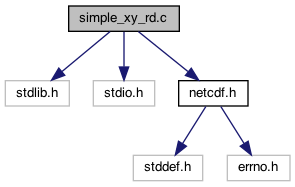
\includegraphics[scale=0.5]{fig/simple__xy__rd_8c__incl}
\end{center}

\end{frame}

\begin{frame}[fragile]{Reading the file \texttt{simple\_xy.nc}}

Create (copy!), compile and run the file \verb|simple_xy_rd.c|\\[0.4cm]

\begin{itemize}

  \item Compile the file \verb|simple_xy_rd.c|

    \begin{itemize}
      \item \footnotesize{ \verb|gcc -I/home/lucy/local/include simple_xy_rd.c -o simple_xy_rd -L/home/lucy/local/lib -lnetcdf| }\\[0.4cm]
    \end{itemize}

  \item Run the file \verb|simple_xy_rd|

    \begin{itemize}
      \item \verb|./simple_xy_rd|
      \item \verb|*** SUCCESS reading example file simple_xy.nc!|

    \end{itemize}

\end{itemize}

\end{frame}

\begin{frame}[fragile]{ncview}

\begin{itemize}

  \item Installation is fine.
  \item What does it do?

\end{itemize}

\end{frame}

\section{File \texttt{simple\_xy\_nc4\_wr.c}}

\begin{frame}[fragile]{}

\begin{itemize}

  \item

\end{itemize}

\end{frame}

\section{File \texttt{simple\_nc4\_wr.c}}

\begin{frame}[fragile]{}

\begin{itemize}

  \item

\end{itemize}

\end{frame}

\section{File \texttt{sfc\_pres\_temp\_wr.c}}

\begin{frame}[fragile]{}

\begin{itemize}

  \item

\end{itemize}

\end{frame}

\section{File \texttt{pres\_temp\_4D\_wr.c}}

\begin{frame}[fragile]{}

\begin{itemize}

  \item

\end{itemize}

\end{frame}

\acknowledgement

\end{document}
